\documentclass[12pt,oneside,a4paper]{article}

\usepackage[utf8]{inputenc} % Lærer LaTeX at forstå unicode - HUSK at filen skal
% være unicode (UTF-8), standard i Linux, ikke i
% Win.

\usepackage[danish]{babel} % Så der fx står Figur og ikke Figure, Resumé og ikke
% Abstract etc. (god at have).

\usepackage{graphicx}
\usepackage{amsfonts}
\usepackage{amsthm}        % Theorems
\usepackage{amsmath}
\usepackage{float}         % Så kan man bedre styre, hvor figurerne havner henne
                           % vha [H].
%\usepackage{hyperref}

%\renewcommand{\mid}[1]{{\rm E}\!\left[#1\right]}
\newcommand{\bas}{\begin{eqnarray*}}
\newcommand{\eas}{\end{eqnarray*}}
\newcommand{\be}{\begin{equation}}
\newcommand{\ee}{\end{equation}}
\newcommand{\bea}{\begin{eqnarray}}
\newcommand{\eea}{\end{eqnarray}}

\newtheorem{thm}{Sætning}[section]
\newtheorem{mydef}[thm]{Definition}
\newtheorem{eks}[thm]{Eksempel}

\DeclareMathSymbol{,}{\mathord}{letters}{"3B}

\title{Lineære modeller}
\date{\vspace{-5ex}}

\begin{document}

\maketitle

%%%%%%%%%%%%%%%%%%%%%%%%%%%%%%%%%%%%%%%%%%%%%%%%%%%%%%%%%%%%%%%%%

\section{Indledning}
Lineære modeller bruges dels til at foretage eksakte omregninger, f.eks. mellem
Fahrenheit og Celsius, og dels til at lave prognoser ud fra kendte data.

Vi begynder med at se på nogle eksempler.

\subsection{Eksempel}
I Europa bruger vi temperaturskalaen Celsius, hvor vand fryser ved 0 grader og
koger ved 100 grader.  I USA bruger de derimod temperaturskalaen Fah\-renheit,
hvor vand fryser ved 32 F og koger ved 212 F.
Man kan omregne mellem de to temperaturskalaer ved følgende formel:
\[
    y = 1,8\cdot x  + 32 \,,
\]
hvor $x$ er temperaturen i grader Celsius og $y$ er temperaturen i Fahrenheit.
Denne sammenhæng er vist grafisk i figuren:

\begin{figure}[H]
    \centering
    \includegraphics[width=0.5\textwidth]{lin-1a}
\end{figure}

Ud fra ligningen er det muligt at omregne mellem temperaturer i Celsius og
temperaturer i Fahrenheit. F.eks.  er kroppens normaltemperatur 37 grader. I
Fahrenheit vil den samme temperatur være
\[
    32 + 1,8\cdot 37 = 98,6\, {\rm F} \,.
\]
På figuren er markeret punkter for kroppens normaltemperatur (37 C,\, 98,6 F) samt
vands kogepunkt (100 C,\, 212 F).

\subsection{Eksempel}
Et teleselskab har et simpelt takstsystem:
\begin{itemize}
    \item Abonnement 5 kr. pr. måned, samt 0,50 kr. pr. talt minut.
\end{itemize}
Hvis en abonnent på en måned taler 25 minutter, skal han betale:
$$
5 + 0,50\cdot25 = 17,50 \, {\rm kr}.
$$
Hvis der tales $x$ minutter en bestemt måned, er prisen $y$ kroner bestemt ved:
$$
y = 5 + 0,50\cdot x \,.
$$
Man siger, at der er en {\em lineær sammenhæng} mellem samtaletiden $x$ og prisen $y$.

Hvis vi afbilder sammenhængen i et koordinatsystem med antallet af minutter på
$x$-aksen og prisen på $y$-aksen, vil sammenhørende værdier af $x$ og $y$ (dvs.
af taletid og pris) udgøre en ret linje med hældning $0,50$, som skærer
$y$-aksen i tallet $5$ (det koster 5 kroner at tale i 0 minutter), se figur
1.1.

\begin{figure}[H]
    \centering
    \includegraphics[width=0.5\textwidth]{lin-1}
\end{figure}

Hældningen $0,50$ angiver prisstigningen for hvert ekstra minut, der tales --
den er 0,50 kroner.  Prisen for 20 minutters samtale er 15 kr., og for 21
minutters samtale er den 15,50 kr.


%%%%%%%%%%%%%%%%%%%%%%%%%%%%%%%%%%%%%%%%%%%%%%%%%%%%%%%%%%%%%%%%%

\section{Lineære sammenhænge}
\begin{mydef}
    En {\em variabelsammenhæng} er en sammenhæng mellem en uafhængig variabel, ofte
    kaldet $x$, og en afhængig variabel, ofte kaldet $y$.
\end{mydef}

En variabelsammenhæng er ofte beskrevet ved en ligning, men kan også tegnes grafisk i et
koordinatsystem.

\begin{mydef}
    En {\em lineær sammenhæng} er en variabelsammenhæng givet ved følgende ligning:
    $$
    y = a\cdot x + b \,,
    $$
    hvor $a$ og $b$ er tal.
\end{mydef}

Vi interesserer os for de koordinatsæt $(x,\,y)$, der passer i en sådan ligning.
Fra folkeskolen ved vi, at sådanne koordinatsæt udgør en ret linje.

Eksempler på sådanne lineære sammenhænge er (se figur 1.2):

\begin{tabular}{ll}
    $\bullet\quad y=3x-5$  & Her er $a=3$ og $b=-5$. \\
    $\bullet\quad y=-2x+1$ & Her er $a=-2$ og $b=1$. \\
    $\bullet\quad y=4-x$   & Her er $a=-1$ og $b=4$. \\
    $\bullet\quad y=3x$    & Her er $a=3$ og $b=0$.
\end{tabular}

\begin{figure}[H]
    \centering
    \includegraphics[width=0.5\textwidth]{lin-2}
\end{figure}

\begin{thm}
    For den lineære sammenhæng
    $$
    y = a\cdot x + b
    $$
    gælder, at grafen er en ret linje, hvor $a$ er linjens {\em hældning} eller
    {\em væksthastghed}.  Det betyder, at linjen vokser med $a$ enheder, når
    $x$ vokser med 1 enhed.  Punktet $(0,\,b)$ er linjens {\em skæringspunkt
    med $y$-aksen}.
\end{thm}

Vi kan opstille en tabel ("sildeben") over koordinater $(x,\,y)$, der passer i
ligningen $y=3x-5$:
$$
\begin{tabular}{c|c|c|c|c|c|c}
    x &  -2 & -1 &  0 &  1 & 2 & 3 \\
    \hline
    y & -11 & -8 & -5 & -2 & 1 & 4
\end{tabular}
$$
Linjen går altså gennem punkterne $(0,\,-5)$, $(1,\,-2)$ osv., se figur 1.3.

\begin{figure}[H]
    \centering
    \includegraphics[width=0.5\textwidth]{lin-3}
\end{figure}

Linjer med samme hældning er parallelle. Linjer med positiv hældning ($a>0$) forløber
opad mod højre, linjer med negativ hældning ($a<0$) nedad mod højre. Linjer med
hældning $a=0$ er vandrette.  Sådanne linjer har en ligning af formen $y=0x+b$
eller blot $y=b$, se figur.

\begin{figure}[H]
    \centering
    \includegraphics[width=0.5\textwidth]{lin-3b}
\end{figure}

Hældningen bestemmes altså ud fra, hvor meget $y$ vokser for hver enhed af $x$. Det
er derfor muligt at aflæse hældningen på grafen ved (fra et valgfrit startpunkt)
at gå 1 til højre og se, hvor meget $y$ stiger eller falder.

Konstanten $b$ afgør, hvor grafen skærer $y$-aksen. Hvis $b$ er positiv finder
skæringen sted over $x$-aksen, og hvis $b$ er negativ er skæringen placeret under $x$-aksen.

At tallet $b$ er linjens skæringspunkt med $y$-aksen følger af, at
koordinatsættet $(0,\,b)$ passer i ligningen:
$$
b = 0\cdot x+b \,.
$$


\subsection{Eksempel}
\begin{figure}[H]
    \centering
    \includegraphics[width=0.5\textwidth]{lin-3a}
\end{figure}

På grafen ovenfor har vi valgt startpunktet $(1,\,1)$. Når vi bevæger
1 til højre, så skal vi gå 2 op for at ramme grafen. Derfor er hældningen $a=2$.
Ligeledes ser vi, at grafen skærer $y$-aksen i punktet $(0,\,-1)$. Derfor er
$b=-1$.
Linjen er derfor beskrevet ved ligningen
\[
    y=2x-1\,.
\]


%Hældningen er illustreret på figur 1.4. Hvis $x$ vokser til $x+1$, så vokser
%$y$ fra $y_1$ til $y_2$ og forskellen $y_2-y_1$ er netop $a$. Bemærk, at $a$
%også kan være negativ, nemlig når $y$ falder i værdi, når $x$ vokser.
%
%\begin{figure}[H]
%    \centering
%    \includegraphics[width=0.5\textwidth]{lin-4}
%\end{figure}


\subsection{Quiz}
\begin{itemize}
    \item Aflæs koordinater af punkter på grafen.
    \item Afgør ved aflæsning om et givet punkt ligger på grafen.
    \item Udregn $y$ ud fra $x$ vha ligningen.
    \item Afgør om et punkt opfylder ligningen.
    \item Aflæs hældningen af en ret linje.
    \item Aflæs skæringen med $y$-aksen.
    \item Aflæs forskriften for en ret linje.
    \item Opskriv ligningen for en linje ud fra en sproglig beskrivelse.
\end{itemize}


%%%%%%%%%%%%%%%%%%%%%%%%%%%%%%%%%%%%%%%%%%%%%%%%%%%%%%%%%%%%%%%%%

\section{Lineær regression}
Ofte, så har man givet en række datapunkter, som ikke ligger på en ret linje. Alligevel
vil man gerne benytte en lineær model, for at kunne foretage prognoser. Vi ser
på et eksempel:

\subsection{Eksempel}
Man har undersøgt højden af et stort antal piger og beregnet middel\-høj\-den for
hver årgang. Pigernes højde ved forskellige aldre fremgår af skemaet.

\[
\begin{array}{|c|c|c|c|c|c|c|c|c|}
    \hline
    \mbox{Alder (år)},\, x &  3 &  4 &  5 &  6 &  7 &  8 & 9 & 10 \\
    \hline
    \mbox{Højde (cm)},\, y &  98,3 &   104,9 &  112,0 &  118,1 &  123,4 &  131,3 & 136,4 & 142,5\\
    \hline
\end{array}
\]

\begin{figure}[H]
    \centering
    \includegraphics[width=0.5\textwidth]{lin-12}
\end{figure}

På figuren ovenfor er punkterne indtegnet, og endvidere er tegnet en {\em
tendenslinje} med ligningen:
\[
    y = 6,31 x + 79,8 \,,
\]
hvor $x$ er alderen i år, og $y$ er pigernes gennemsnitlige højde i cm.

Det ses, at linjen følger punkterne med rimelighed. Det er derfor muligt at
bruge ligningen for den rette linje til at foretage pronoser. F.eks. kan man
forudsige en piges gennemsnitlige højde ved alderen 12 år ved at indsætte $x=12$
i ligningen. Det giver
\[
    y=6,31\cdot 12 + 79,8 = 155,5 \mbox{ cm. }
\]
Altså forudsiger denne model, at piger i alderen 12 år har en gennemsnitlig
højde på 155,5 cm.  Det skal understreges, at der en tale om en prognose, som
bygger på en række forudsætninger.  I dette tilfælde forudsætter modellen,
fordi det er en {\em lineær} model, at piger vokser med det samme antal cm
hvert år, i dette tilfælde 6,31 cm.

Denne forudsætning holder ikke, når pigernes alder passerer puberteten.
Endvidere er der tale om et gennemsnit.  Alligevel bliver sådanne modeller brugt
i stor udstrækning, og det er derfor vigtigt at kende modellernes
forudsætninger. 
\begin{thm}
    I en lineær model forudsættes det, at væksthastigheden er konstant.
\end{thm}

\subsection{Mindste kvadraters metode}

For at finde frem til tendenslinjen, som er den linje, der bedst bestemmer
punkterne, benytter man som regel et CAS-værktøj. I dette afsnit forklares,
hvordan tendenslinjen udvælges.

CAS-værktøjer benytter sædvanligvis en metode, der kaldes {\em mindste
kvadraters metode}.

\begin{figure}[H]
    \centering
    \includegraphics[width=0.5\textwidth]{lin-11}
\end{figure}

På figuren er en række punkter afsat, og en vilkårlig linje $m$ er tegnet.
Desuden er de lodrette afstande $d_1$, $d_2$, $d_3$, ..., $d_n$ fra
målepunkterne til linjen afsat, samt de tilhørende kvadrater. Man kan så
udregne summen $D$ af kvadraternes areal:

\[
D = {d_1}^2 + {d_2}^2 + {d_3}^2 + \ldots + {d_n}^2 \; . 
\]

Hvis man vælger en anden linje, får man selvfølgelig i reglen en anden kvadratsum.

Man har vedtaget at den linje, der gør kvadratsummen $D$ mindst mulig, er den
'bedste' linje. Metoden kaldes {\em de mindste kvadraters metode}, og den linje, der
fremkommer, kaldes {\em regressionslinjen} eller {\em tendenslinjen} svarende
til punkterne. Vi går ikke ind på, hvordan linjen matematisk bestemmes. 

\subsection{Korrelation}
CAS giver foruden regressionslinjens ligning den såkaldte {\em
korrelations\-koef\-fi\-cient} $r$. Vi kommer ikke her ind på teorien bag
beregningen af dette tal, men nøjes med at bemærke, at
korrelationskoefficienten er et mål for den lineære sammenhæng mellem
punkterne.

Vi bemærker følgende om korrelationskoefficienten $r$:

\begin{itemize}
    \item Hvis $r = 1$ ligger punkterne præcis på ret linje med positiv hældning.
    \item Hvis $0 < r < 1$ har regressionslinjen positiv hældning. Jo tættere $r$
        er på 1, desto tættere ligger punkterne på linjen.
    \item Hvis $r = 0$ eller tæt ved 0, er der ingen eller kun svag lineær sammenhæng.
    \item Hvis $-1 < r < 0$ har regressionslinjen negativ hældning. Jo tættere $r$
        er på -1, desto tættere ligger punkterne på linjen.
    \item Hvis $r = -1$ ligger punkterne præcis på ret linje med negativ hældning. 
\end{itemize}
På næste figur er disse forhold illustreret.

\begin{figure}[H]
    \centering
    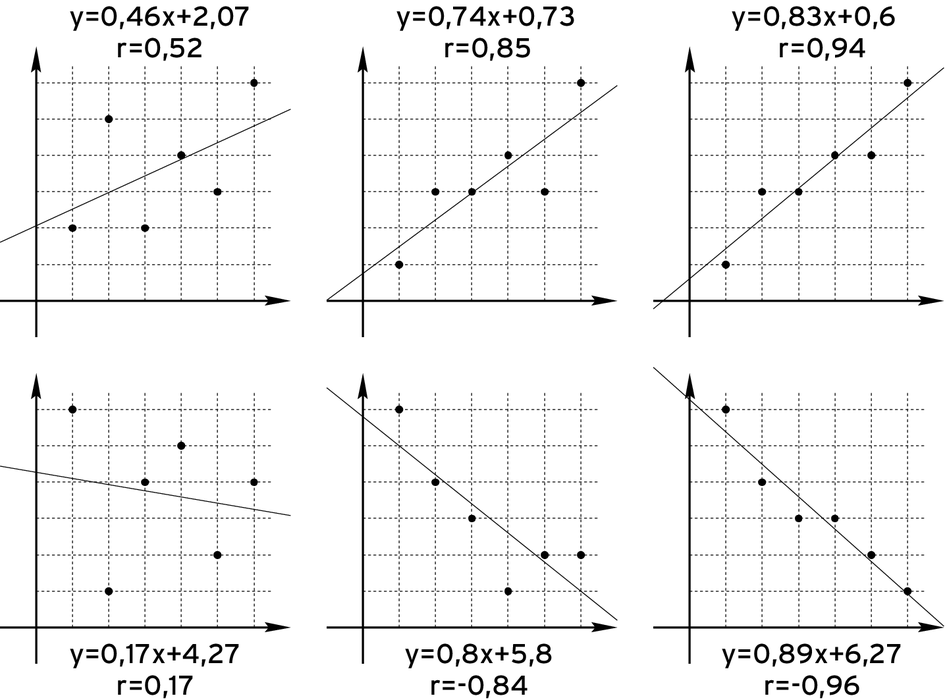
\includegraphics[width=\textwidth]{fig57}
\end{figure}

\subsection{Eksempel}
I et fysikforsøg måles vægt og rumfang at et måleglas med sand. Det giver følgende værdier:

\[
\begin{array}{|c|c|c|c|c|c|}
    \hline
    \mbox{Rumfang (ml)},\, x &  50 &  100 &  150 &  200 &  250  \\
    \hline
    \mbox{Vægt (g)},\, y &  225 &   305 &  380 &  465 &  540 \\
    \hline
\end{array}
\]
hvor $x$ er rumfanget i ml, og $y$ er vægten i gram.

Målinger er vist i den følgende figur:

\begin{figure}[H]
    \centering
    \includegraphics[width=0.5\textwidth]{lin-11a}
\end{figure}

På figuren er også indtegnet tendenslinjen givet ved ligningen
\[
    y=1,58 x + 146 \,.
\]

Punkterne passer overordentligt godt med linjen, og vi kan derfor sige, at linjen er en god model
til at beskrive sammenhængen mellem vægt og rumfang i dette forsøg.

Endvidere kan vi fortolke konstanterne $1,58$ og $146$ i modellen på følgende måde:
\begin{itemize}
    \item Konstanten $1,58$ angiver, hvor meget vægten stiger, når rumfanget af
        sandet øges med 1 ml. Dette er det samme som sandets densitet
        (massefylde), som i dette forsøg er bestemt til $1,58$ g/ml.
    \item Konstanten $146$ er vægten, når måleglasset er tomt. Det vil sige, at
        i dette forsøg er vægten af det tomme måleglas bestemt til $146$ gram.
\end{itemize}

Forklaringsgraden er af CAS-værktøjet angivet til at være $r=0,9998$, hvilket bekræfter, at modellen
passer særdeles godt med målingerne. Derfor er det rimeligt at konkludere, at der er en 
lineær sammenhæng mellem rumfang og vægt af sand, og at sandets densitet er konstant.

\subsection{Eksempel}
Fra statistikbanken.dk kan man finde data over "tilskadekomne og dræbte i spiritusuheld" i Danmark, som
angivet i følgende tabel:

\[
\begin{array}{|c|c|c|}
    \hline
    $x$ & \mbox{årstal} & \mbox{antal} \\
    \hline
    0 & 2007 & 1261 \\
    \hline
    1 & 2008 & 1012 \\
    \hline
    2 & 2009 & 861 \\
    \hline
    3 & 2010 & 671 \\
    \hline
    4 & 2011 & 698 \\
    \hline
    5 & 2012 & 548 \\
    \hline
    6 & 2013 & 504 \\
    \hline
    7 & 2014 & 417 \\
    \hline
    8 & 2015 & 384 \\
    \hline
\end{array}
\]

Generelt, når $x$-aksen består af årstal, så vælger man oftest at sætte $x=0$ ved det første årstal.
Det vil sige, at
\[
    x = \mbox{årstal} - 2007\,.
\]
Dette er ligeledes angivet i tabellen oven over.

På figuren er ovenstående punkter indsat, sammen med en ret linje.

\begin{figure}[H]
    \centering
    \includegraphics[width=0.5\textwidth]{lin-11b}
\end{figure}

Tendenslinjen er udregnet på CAS værktøj til
\[
    y=-102,2x+1115 \,.
\]

Punkterne passer nogenlunde med linjen, og vi kan derfor med et vist forbehold
sige, at der er en tilnærmelsesvis lineær sammanhæng mellem årstal og antal
tilskadekomne og dræbte i spiritusuheld i Danmark.

Forklaringsgraden er $-0,9597$ er tæt på $-1$, og antyder en generel overensstemmelse mellem
data og model.

Konstanterne $-102,2$ og $1115$ i modellen kan fortolkes på følgende måde:
\begin{itemize}
    \item Konstanten $-102,2$ angiver, at for hvert år reduceres antallet
        af tilskadekomne og dræbte i spiritusuheld i Danmark med ca. 102 personer.
    \item Konstanten $1115$ fortæller, at der ved modellens begyndelse, dvs i år 2007,
        var 1115 tilskadekomne og dræbte i spiritusuheld i Danmark. Det passer åbenlyst
        ikke med det rigtige antal på 1261 personer i tabellen oven over. Forskellen er
        et udtryk for, at modellen afviger fra de faktiske antal.
\end{itemize}

Denne lineære model har dog en indbygget svaghed, nemlig at antal personer fortsætter med at falde.
På et tidspunkt (efter ca. yderligere fire år) vil modellen angive et negativt antal personer, hvilket 
er åbenlyst forkert. Så ligesome i det tidligere eksempel med pigers højde, så er modellens
anvenlighed begrænset.

\subsection{Quiz}
\begin{itemize}
    \item Give en fornuftig fortolkning $a$, $b$ og $r$ ud fra en given model.
    \item Forholde sig kritisk til en models gyldighedsområde.
\end{itemize}

%%%%%%%%%%%%%%%%%%%%%%%%%%%%%%%%%%%%%%%%%%%%%%%%%%%%%%%%%%%%%%%%%

\section{Løsning af førstegradsligninger}
En ligning er af første grad, hvis den er af typen
$$
ax + b = 0\; ,
$$
eller umiddelbart kan omskrives til en sådan ligning. Her er et par eksempler:
$$
3x - 4 = 8 + 2x \quad , \quad 5(x - 4) + 2x = 6x - 2(3 - 4x)\; .
$$

\subsection{Ensbetydende ligninger}
Hvis man foretager en række omformninger af en ligning for at finde en løsning,
bruger man symbolet $\Leftrightarrow$ , en dobbeltpil (eller en {\em
biimplikation}), mellem ligninger, der har de samme løsninger. Fx har vi
\bas
&& 2(3x - 1) = x - 4(2 - x)\\
&\Leftrightarrow& 6x - 2 = x - 8 + 4x\\
&\Leftrightarrow& 6x - 2 = 5x - 8 \\
&\Leftrightarrow& x = -6 
\eas
Hver af de fire ligninger har den samme løsning. Man siger, at sådanne
ligninger er {\em ensbetydende}. Man kan også sige, at ensbetydende ligninger
fremgår af hinanden ved ’lovlige’ omformninger.

Vi anfører de vigtigste regler for løsning af ligninger.

[ANIMATION OM REGNEREGLER 1--4]

\subsection{Eksempel}
Førstegradsligninger optræder ofte i forbindelse med lineære modeller. F.eks. i
eksemplet med dræbte og tilskadekomne kan man beregne, hvornår modellen
forudsiger, at antallet er lig med 0.  Efter dette tidspunkt bliver antallet
negativt, og så giver modellen ikke længere mening.  Vi skal da løse følgende
ligning:
\[
\begin{aligned}
    & -102,2x+1115 = 0  \\
    \iff & -102,2x = -1115 \\
    \iff & x = \frac{-1115}{-102,2} \\
    \iff & x = 10,9
\end{aligned}
\]
Svaret $x=10,9$ skal forstås således, at i år $x + 2007 = 10,9 + 2007 = 2017,9$
vil antallet af dræbte og tilskadekomne blive lig med nul. Modellen her derfor
højst gyldighed frem til år 2017.


\subsection{Quiz}
\begin{itemize}
    \item Løse ligningen $5x+7 = 0$
    \item Løse ligningen $-5x+7 = 0$
\end{itemize}


%%%%%%%%%%%%%%%%%%%%%%%%%%%%%%%%%%%%%%%%%%%%%%%%%%%%%%%%%%%%%%%%%

\section{Skæring mellem linjer}
Hvis to linjers ligninger er kendt, vil vi finde koordinaterne til linjernes
skæringspunkt (hvis de ikke er parallelle).

Linjerne $l$ og $m$ har f.eks. ligningerne (se figur 2.9)
\[
    l: y=0,5x-2\quad{\mbox{og}}\quad m: y=-3x+5 \,.
\]

\begin{figure}[H]
    \centering
    \includegraphics[width=0.5\textwidth]{lin-9}
\end{figure}

I skæringspunktet mellem linjerne skal $y$-værdien for de to linjer være den
samme, så der må gælde, at
\[
0,5x-2 = -3x+5 \,,
\]
og denne ligning løses på følgende måde:
\bas
&& 0,5x+3x=5+2\\
&\iff& 3,5x=7\\
&\iff& x=2
\eas
Denne værdi af $x$ indsættes i en af ligningerne, ligegyldig hvilken:
\[
y=0,5\cdot2-2=-1 \,.
\]
Skæringspunktet har altså koordinaterne $(2,\,-1)$, hvilket ser ud til at
stemme med figuren.

\subsection{Eksempel}
Skæring mellem linjer optræder typisk, når man vil sammenligne to forskellige
modeller.  I indledningen betragtede vi et teleselskab, hvor prisen pr. måned
kunne beskrives ved følgende ligning
\[
    y = 5 + 0,50 \cdot x \quad \mbox{selskab A}\,,
\]
hvor $x$ er den samlede samtaletid i løbet af måneden, og $y$ er den samlede
pris. Her er konstanten $0,50$ prisen pr. minut, og konstanten $5$ er den faste
abonnementspris om måneden, uafhængig af samtaletiden.

Nu vil vi sammenligne dette med et andet teleselskab, som godt nok har et højere abonnnement,
men til gengæld en lavere minutpris. Vi ser således på
\[
    y = 10 + 0,20 \cdot x \quad \mbox{selskab B}\,.
\]
Ved et lavt forbrug vil selskab B være for dyrt, men hvis forbruget er meget stort, så vil
selskab B være billigst.

Vi kan nu undersøge, ved hvilket forbrug de to selskaber vil være lige dyre. Vi skal 
altså finde skæringspunktet mellem de to rette linjer, se figuren:
\begin{figure}[H]
    \centering
    \includegraphics[width=0.5\textwidth]{lin-9a}
\end{figure}
Af figuren fremgår det, at ved et forbrug på ca. 17 minutter om måneden er de to selskaber
lige dyre. Vi kan beregne denne pris ved at løse følgende ligning:
\[
\begin{aligned}
    & 5 + 0,50 x = 10 + 0,20 x \\
    \iff & 0,30x = 5 \\
    \iff & x = 16,67
\end{aligned}
\]
Så ved et forbrug over $16,67$ minutter vil selskab B være at foretrække.

\subsection{Quiz}
\begin{itemize}
    \item Løs ligningen $5x+7 = 2x+3$
    \item Løs ligningen $-5x+7 = 2x+3$
\end{itemize}


%%%%%%%%%%%%%%%%%%%%%%%%%%%%%%%%%%%%%%%%%%%%%%%%%%%%%%%%%%%%%%%%%

\section{Ligefrem proportionalitet}
Man bruger den talemåde, at to variabler $x$ og $y$ er {\em ligefrem
proportionale} (eller blot: {\em proportionale}), hvis de "stiger og falder i
samme takt". Vi skal se på, hvad denne lidt løse udtalelse dækker over.

Hvis en bil kører med konstant hastighed, f.eks. 90 km/t, kan vi opstille en
tabel over sammenhængen mellem tiden $x$ og den tilbagelagte afstand $y$:
\[
\begin{tabular}{c|c|c|c|c|c|c}
    x ({\rm min}) & 10 & 20 & 30 & 40 & 60 & 120 \\
    \hline
    y ({\rm km})  & 15 & 30 & 45 & 60 & 90 & 180  
\end{tabular}
\]
Vi ser, at $y$ netop er $1,5$ gange så stor som $x$, så sammenhængen mellem $x$
og $y$ kan udtrykkes som
\[
y = 1,5\cdot x
\]
Talemåden "$y$ ændrer sig i samme takt som $x$" betyder netop, at $x$ skal
ganges med et fast tal (her $1,5$) for at give $y$. Man kan også udtrykke det
sådan:
\begin{itemize}
    \item Når $x$ bliver dobbelt så stor, bliver $y$ også dobbelt så stor.
    \item Når $x$ bliver tre gange så stor, bliver $y$ også tre gange så stor.
    \item Når $x$ bliver halvt så stor, bliver $y$ også halvt så stor.
    \item osv.
\end{itemize}
Hvis man med konstant hastighed kører dobbelt så lang tid, tilbagelægger man
også dobbelt så lang afstand, se figur 3.6.

\begin{figure}[H]
    \centering
    \includegraphics[width=0.5\textwidth]{lin-5}
    \caption{Figur 2.5}
    \label{fig36}
\end{figure}

I dette tilfælde er tidsrummet $x$ og afstanden $y$ proportionale, og tallet
$1,5$ kaldes {\em proportionalitetsfaktoren}, fordi det netop er en faktor foran $x$.

Man kan også sige, at forholdet mellem $y$ og $x$ er konstant, fordi vi får:
\[
y = 1,5\cdot x \, \Leftrightarrow \, \frac{y}{x} = 1,5
\]
Forholdet mellem afstand og tid kaldes hastighed, og tallet angiver her netop
hastigheden: bilen kører med en hastighed på $1,5$ km/min, svarende til $90$
km/t.

Sammenhængen illustreres som en ret linje gennem $(0,\,0)$ med hældningen $1,5$.

\begin{mydef}
    To variabler $x$ og $y$ kaldes proportionale, hvis der findes et tal $k$, så
    $$
    y = k\cdot x \,\, {\rm eller} \,\, \frac{y}{x} = k
    $$
    Tallet $k$ kaldes proportionalitetsfaktoren. Sammenhængen mellem $x$ og $y$
    illustreres i koordinatsystemet af en ret linje gennem $(0,\,0)$ med 
    hældning $k$.
\end{mydef}

En proportional sammenhæng er således et specialtilfælde af en lineær sammenhæng, hvor
skæringen med $y$-aksen er $b=0$.

\subsection{Eksempel (sammenhæng mellem masse og volumen)}

Et eksempel på ligefrem proportionalitet er sammenhængen mellem masse og rumfang af olie.
Der gælder nemlig, at en liter olie vejer 0,8 kg. To liter olie vejer derfor 1,6 kg,
og generelt vejer $x$ liter olie $y$ kg, hvor
\[
y = 0,8 \cdot x \,.
\]
Tallet $0,8$ er således vægten af én liter olie og det kaldes for oliens
massefylde.  At olie flyder oven på vand skyldes netop, at oliens massefylde er
mindre end vands.

\subsection{Eksempel}
I eksempel 1.1 så vi på teleselskabet, hvor prisen $y$ (naturligvis) afhænger af
taletiden $x$ i minutter:
\[
y=20+0,5x \,.
\]
Her er prisen ikke proportional med taletiden: Dobbelt så lang taletid koster ikke
det dobbelte:
\begin{itemize}
    \item 15 minutter koster $20+0,5\cdot 15 = 27,50$ kroner.
    \item 30 minutter koster $20+0,5\cdot 30 = 35,00$ kroner.
\end{itemize}
I koordinatsystemet går linjen med ligningen $y=20+0,5x$ nemlig ikke gennem $(0, 0)$,
sådan som kravet til proportionalitet er.

\subsection{Quiz}
\begin{itemize}
    \item Bestem forskrift ud fra sproglig fremstilling.
    \item Bestem forskrift ud fra et givet punkt.
\end{itemize}

%%%%%%%%%%%%%%%%%%%%%%%%%%%%%%%%%%%%%%%%%%%%%%%%%%%%%%%%%%%%%%%%%

\section{Linje gennem to punkter}
Vi vil bestemme hældningen for en linje, der går gennem
to punkter med kendte koordinater, se figuren. Vi viser følgende sætning:
\begin{thm}
    Hvis $A(x_1,\,y_1)$ og $B(x_2,\,y_2)$ er to punkter på en ret linje, der ikke
    er lodret, dvs $x_1\neq x_2$, er hældningen $a$ af linjen bestemt ved
    $$
    a = \frac{y_2-y_1}{x_2-x_1}
    $$
\end{thm}

\begin{figure}[H]
    \centering
    \includegraphics[width=0.5\textwidth]{lin-6}
    \label{linear-1}
\end{figure}

\begin{proof}
    Linjens ligning er
    $$
    y = a\cdot x + b.
    $$
    De punkter, som ligger på linjen, har koordinater, der passer i
    ligningen.  Da $A$ og $B$ ligger på linjen, passer deres koordinater altså
    i ligningen, dvs.
    $$
    y_1 = a\cdot x_1 + b \quad {\rm og} \quad y_2 = a\cdot x_2 + b 
    $$
    Vi trækker den første ligning fra den sidste og får
    \bas
    y_2 - y_1 &=& a\cdot x_2 + b - (a\cdot x_1 + b) \\
              &=& a\cdot x_2 - a\cdot x_1 \\
              &=& a\cdot \left(x_2-x_1\right) 
    \eas
    altså $y_2-y_1 = a \cdot \left(x_2-x_1\right)$, hvoraf
    $$
    a = \frac{y_2-y_1}{x_2-x_1}
    $$
    og det var netop, hvad vi ville vise.
\end{proof}

Læg mærke til, at vi i den sidste ligning har divideret med tallet $x_2-x_1$ på
begge sider af lighedstegnet. Dette tal er nemlig ikke $0$, fordi $x_1$ og
$x_2$ er forskellige tal -- vi har jo netop forudsat, at linjen ikke er lodret, se
figuren.

\begin{figure}[H]
    \centering
    \includegraphics[width=0.5\textwidth]{lin-7}
    \label{linear-2}
\end{figure}

I formlen for hældningen $a$ angiver tælleren $y_2-y_1$ den lodrette afstand
mellem punkterne $A$ og $B$, mens nævneren $x_2-x_1$ angiver den vandrette
afstand. Vi kan derfor lidt populært sige, at
\[
a = \pm \frac{\mbox{lodret afstand}}{\mbox{vandret afstand}} \,.
\]
Her står $\pm$ for at minde om, at der skal anbringes et minus foran brøken,
hvis hældningen er negativ.
\begin{eks}
    Vi ser på linjen $l$ gennem $A(-1,\,3)$ og $B(4,\,5)$.
    Linjens hældning er
    $$
    a = \frac{5-3}{4-(-1)} = \frac{2}{5} = 0,4.
    $$
    Skæringspunktet med $y$-aksen finder vi ved at indsætte det ene punkts
    koordinater i ligningen:
    $$
    5 = 0,4\cdot 4 + b.
    $$
    Det giver
    $$
    b = 5 - 0,4\cdot 4 = 3,4.
    $$
    Linjens ligning er dermed
    $$
    y = 0,4 \cdot x + 3,4 
    $$
\end{eks}
\begin{figure}[H]
    \centering
    \includegraphics[width=0.5\textwidth]{lin-8}
    \label{linear-3}
\end{figure}


\begin{thm}
    Hvis $A(x_1,\,y_1)$ er et punkt på en ret linje, og linjen har hældningen
    $a$, så er linjens ligning givet ved
    $$
    y = a\cdot (x-x_1) + y_1 
    $$
\end{thm}
\begin{proof}
    Vi har generelt, at 
    $$
    y = a\cdot x + b
    $$
    og i punnket $(x_1, y_1)$ gælder:
    $$
    y_1 = a\cdot x_1 + b
    $$
    Trækkes den nederste ligning fra den øverste får vi:
    $$
    y-y_1 = a \cdot x + b - (a \cdot x_1 + b)
    $$
    $$
    \Leftrightarrow y-y_1 = a \cdot x - a \cdot x_1
    $$
    $$
    \Leftrightarrow y-y_1 = a \cdot (x - x_1)
    $$
    Dermed har vi vist det ønskede.
\end{proof}

\subsection{Quiz}
\begin{itemize}
    \item Bestem hældning af linje gennem to givne punkter.
    \item Bestem forskrift for linje gennem to givne punkter.
    \item Kontrollere, at en given forskrift går gennem to givne punkter.
\end{itemize}

\end{document}

